\documentclass{article}

\usepackage{amsmath,amssymb}
\usepackage{enumerate}
\usepackage{nips12submit_e}
\usepackage{times}
\usepackage{url}
\usepackage{graphicx}

\nipsfinalcopy

\title{Faster Unsupervised Morphology Induction}

\author{
Victor Chahuneau\\
\texttt{vchahune@cs.cmu.edu}
\And
Phani Gadde\\
\texttt{pgadde@cs.cmu.edu} \\
\And
Peter Schulam\\
\texttt{pschulam@cs.cmu.edu}
}

\begin{document}

\maketitle

\section{Introduction}

Building accurate morphological analyzers is a time-consuming task,
which requires linguistic knowledge and abilities to formalize
morphological phenomena into finite-state rules. This approach has
been successful for several European languages, but the majority of
languages still lack such resources. Unsupervised methods are
therefore an interesting alternative that has been extensively
explored and several approaches -- mostly based on
information-theoretic criteria (MDL) -- have been proposed to solve
this problem. Recently, probabilistic models making use of
non-parametric Bayesian techniques have shown competitive performance.

In particular, Goldwater \& al. \cite{goldwater2011} propose a
baseline model for modeling types and tokens in morphological
induction. Lee \& al. \cite{lee2011} suggest an extension which takes
context into account, while Dreyer \& Eisner \cite{dreyer2011} add
structure by encoding morphological phenomena into paradigms that are
tied to grammatical functions, but evaluate their model in a
semi-supervised setting.

Unsupervised morphological analysis is typically done using complex
nonparametric Bayesian models. Deriving the posterior distribution
over quantities of interest (such as the stem lexicon of a language)
can yield complex mathematical expressions which are difficult to
compute. In some applications of Bayesian statistical modeling, it is
acceptable to run samplers for a long time in order to compute a
useful result, but in natural language processing, and, more
specifically, morphological analysis, the amount of data that must be
processed is often large. Furthermore, as morphological analysis is
typically a step used to preprocess tokens in a document before
applying other types of linguistic analysis, it is not a process on
which we would like to spend too much time.

Crude morphological analysis tools such as the Porter Stemmer are easy
to implement and computationally inexpensive, and thus have been
successful in areas such as information retrieval where we need to
quickly ``analyze'' billions of tokens. Recent Bayesian morphological
models are more linguistically sophisticated, and could potentially
provide more accurate stemming information. Real world application of
these models is not realistic, however, due to the long running time
required when using MCMC methods for inference. Our project aims to
integrate recent advances in speeding up MCMC computation into one of
the fundamental Bayesian morphological models. Our goals are to:

\begin{enumerate}[1.]
\item Reparameterize the model proposed in \cite{goldwater2011} so
  that inference can be distributed.
\item Implement the reparameterization.
\item Evaluate timing and performance differences between original
  model and our reparameterization.
\end{enumerate}

In the baseline model proposed in \cite{goldwater2011}, the 
generator distribution is a joint on the inflectional classes, stems 
and affixes. The adaptor is the PYCRP in which each customer represents 
a word token and each table is labeled with a lexical item. The sampling 
process involves doing the following two steps iteratively.

\begin{enumerate}[1.]
\item Sampling a new morphological analysis for the label on each table,
fixing the assignment of words to tables
\item Re-assigning each word to a new table, fixing the morphological analyses
\end{enumerate}

Step 2 above iterates through every word token in the corpus and computes
the distribution over table assignments for that token conditioning on 
the table assignments for all the other tokens. Since we need know the 
table assignments for all the words to sample a table for each word, this
step cannot be done in parallel with a simple partitioning of data points. 
At the same time, this is the most time consuming task in the sampling. 
Our goal is to parallelize these two steps to speed-up the inference.

Parallelizing inference is related the conditional independencies in the 
model. One way to achieve more independencies is by optimizing a variational 
approximation of the posterior. However, we lose the expressiveness of the 
model in such cases. \cite{asuncion2008asynchronous} proposed an approximate
distributed Gibbs sampler for HDP that works on a given set of $P$ processors.
Each processor updates 1/$P$ cluster allocations and global allocations are 
used for the observations not stored on any local processor. The cluster
allocations are amalgamated in the synchronization step that follows the 
distributed Gibbs steps. These approaches, by construction, optimize an 
approximation of the desired objective and hence are less preferred.

\cite{lovell2012,williamsonparallel} proposed exact inference methods
for parallelizing DP mixture models. Williamson et. al \cite{williamsonparallel}
 use the fact that for appropriate parameter settings, Dirichlet mixtures of
Dirichlet processes are Dirichlet processes. They perform MCMC for an equivalent
equilibrium distribution from $P$ distributed DPs. Lovell et. al \cite{lovell2012}
 reparameterize the DP to induce conditional independencies between the 
distributed DPs. We use a similar reparameterization for our morphology
model thereby parallelizing the inference without approximations.

Our contributions in this paper are reparameterizing the baseline model
 from \cite{goldwater2011} following \cite{lovell2012} and 
implementing it using a parallel architecture on a single core.

\section{Related Work}
\label{sec:related-work}

\subsection{Parallel Markov Chain Monte Carlo for Dirichlet Process Mixtures}
\label{sec:parallel-mcmc-for-dpm}

\cite{lovell2012} propose a reparameterization of Dirichlet Process
mixture models that allows MCMC inference schemes to be split across
multiple machines. The high-level strategy is to form
``superclusters'' of latent variable labels so that latent variables
for each data point $x_i$ within a supercluster are conditionally
independent of other data points given the supercluster
assignments. This allows the most expensive piece of the computation
(sampling the posterior distribution over latent labels) to be
performed in parallel within each supercluster. We review their
contribution as we derive our reparameterization of
\cite{goldwater2011} from it.

\cite{lovell2012} define the following generative process, which, as
we will show, defines the same target distribution as an unmodified
Dirichlet process with concentration parameter $\alpha$ and base
distribution $H$. We begin by drawing a sample $\boldsymbol{\mu}$ from
a distribution over the $K$ dimensional simplex, where $K$ is the
number of superclusters that we would like in our model. Functionally,
this defines the number of compute nodes over which we would like to
distribute our computation. We now draw another vector
$\boldsymbol{\gamma}$ from the $K$ dimensional simplex, but now draw
from the Dirichlet distribution with parameters $\alpha \mu_1, \ldots,
\alpha \mu_K$. We know draw $K$ random distributions from $K$
independent Dirichlet processes with the base measure $H$. Each of the
Dirichlet processes has concentration parameter $\alpha \mu_i$ where
$i \in \{1, \ldots, K\}$. Finally, we form a distribution $G$ by
mixing $G_1, \ldots, G_k$ with weights $\gamma_1, \ldots,
\gamma_K$. The full generative process is as follows:

\begin{align*}
  \mu_1, \ldots, \mu_K &\sim Dirichlet(\tau) \\
  \gamma_1, \ldots, \gamma_K &\sim Dirichlet(\alpha \mu_1, \ldots, \alpha \mu_K) \\
  G_i &\sim DP(\alpha \mu_i, H) \text{ for } i \in \{1, \ldots, K\} \\
  G &= \sum_{i=1}^K \gamma_i G_i
\end{align*}

They authors of \cite{lovell2012} note that the procedure defined
above results in $G \sim DP(\alpha, H)$. The key property of this
reparameterization of the Dirichlet process is that the standard
Chinese Restaurant Process gets reformulated as a two-stage process in
which a new data point first chooses which restaurant it will eat at,
and then chooses a table based on where other customers of that
restaurant are seated.

We now go through the mathematics of the process in more detail. We
follow the original paper, using $z_n$ to denote the table chosen by
the $n$th data point where $n$ ranges from $\{1, \ldots, N\}$. We let
$j \in \mathbb{N}$ uniquely index the tables across \textit{all}
restaurants, and $s_j = i$ be the supercluster or restaurant in which
the $j$th table is located. We can then express the probability that a
customer chooses restaurant $i$ given $\alpha$ as

\begin{align}
  Pr(s_{z_n} = i | \{z_{n^\prime}\}_{n^{\prime}=1}^{n-1}, \alpha)
  &= \frac{\alpha \mu_i + \sum_{n^\prime = 1}^{n-1} \mathbb{I}(s_{z_{n^\prime}} = i)}{\alpha + n - 1}
\end{align}

This is simply the predictive probability of restaurant $i$ under the
Dirichlet multinomial with prior $Dir(\alpha\boldsymbol{\mu})$. Once a
customer has chosen restaurant $i$, then she chooses a table within
the restaurant according to a local Chinese Restaurant Process

\begin{align}
  P(z_n = j, 1 \le j \le \#tables(i) | \{z_{n^\prime}\}_{n^{\prime}=1}^{n-1}, \alpha, s_j = i)
  &= \frac{\sum_{n^\prime = 1}^{n-1} \mathbb{I}(s_{z_{n^\prime}} = i, z_{n^\prime} = j)}
          {\alpha \mu_i + \sum_{n^\prime = 1}^{n-1} \mathbb{I}(s_{z_{n^\prime}} = i)} \\
  P(z_n = j, j = \#tables(i) + 1 | \{z_{n^\prime}\}_{n^{\prime}=1}^{n-1}, \alpha, s_j = i)
  &= \frac{\alpha \mu_i}{\alpha \mu_i + \sum_{n^\prime = 1}^{n-1} \mathbb{I}(s_{z_{n^\prime}} = i)}
\end{align}

The key property of the expressions above that allow us to parallelize
the MCMC inference algorithm is that the probability of a customer
sitting at a table $j$ conditioned on the restaurant $i$ is
independent of all customers that are not seated at that restaurant
(since the sums in both the numerator and denominator in the first
expression and the denominator in the second expression do not count
$s_{z_{n^\prime}} \neq i$). Therefore, when resampling seating
arrangements, which is often the most computationally intensive aspect
of MCMC in Dirichlet process mixture models, we can reseat customers
in each restaurant on different compute nodes.

\subsection{Transition Operators}
\label{sec:parallel-transition-operators}

Following \cite{lovell2012}, we define the following relevant counts

\begin{align*}
  \#i = \sum_{n=1}^N \mathbb{I}(s_{z_n} = i),\text{ }
  \#j = \sum_{n=1}^N \mathbb{I}(z_n = j),\text{ }
  J_i = \sum_{j=1}^\infty \mathbb{I}(\#k > 0, s_j = i)
\end{align*}

We now discuss the distributions from which each variable in the model
described above can be sampled. This includes $\alpha$ (the
concentration parameter of the primary Dirichlet process), $z_n$ (the
seating arrangements of the customers), and $s_j$ (the restaurant
assignment for each cluster $j$). Note that we do not discuss the
model parameters $\theta_j$ for each cluster $j$. \cite{lovell2012} do
not devote much attention to this and briefly mention that this is
model specific, but can sometimes be done in parallel. For our model
of morphology, however, this is not the case. Indeed, the models of
morphology that we use require global knowledge of the current
analysis for types in the corpus. We therefore put discussion of the
model-specific parameters off until the next section.

The first parameter we can resample is the concentration
$\alpha$. This should be resampled conditioned on the seating
arrangements $\{z_n\}_{n=1}^N$. Assuming a prior $\pi(\alpha)$, the
posterior over $\alpha$ is

\begin{align}
  p(\alpha | \{z_n\}_{n=1}^N) \propto p(\alpha) p(\{z_n\}_{n=1}^N | \alpha)
\end{align}

\cite{lovell2012} show that the likelihood of the seating arrangements
and the cluster assignments to restaurants can be expressed as

\begin{align}
  P(\{z_n\}_{n=1}^N, \{s_j\}_{j=1}^\infty | \alpha) &=
  \frac{\Gamma(\alpha)}{\Gamma(N + \alpha)} \alpha^{\sum_{i=1}^K J_i \prod_{i=1}^K \mu_i^{J_i}}
\end{align}

which is simply the marginal Chinese Restaurant Process multipled by
an additional factor that accounts for how the clusters are assigned
to each restaurant (i.e. the supercluster assignments). This allows us
to then rewrite the posterior over $\alpha$ as

\begin{align}
  p(\alpha | \{z_n\}_{n=1}^N) \propto p(\alpha) \frac{\Gamma(\alpha)}{\Gamma(N + \alpha)} \alpha^{\sum_{i=1}^K J_i \prod_{i=1}^K \mu_i^{J_i}}
\end{align}

Resampling the seating assignments $z_n$ given the restaurant
assignments $s_j$, model-specific parameters $\theta_j$, and
concentration $\alpha$ can be done exactly as it is done in the
standard Chinese Restaurant Process. The primary difference, as
explained above, is that the distribution over tables for a particular
customer given the restaurant assignment is independent of all
customers that are not eating at that restaurant. This allows us to do
sampling for each restaurant in parallel, which can significantly
speed up inference. \cite{lovell2012} also note that since each local
CRP is no different from standard CRP sampling, techniques used to
improve sampling speed for standard CRPs (e.g. \cite{neal2000},
\cite{walker2007}, and \cite{papaspiliopoulos2008}) can be applied to
get further gains in speed.

\section{Proposed Method}
\label{sec:proposed-method}

\subsection{Morphology induction model}

We follow \cite{goldwater2011} in describing a basic model for
learning morphological analysis from a corpus of words. The generative
story can be divided into two steps: first, generating a lexicon of
words by putting together stems and suffixes based on a word class
distribution; and secondly, generating sequences of tokens taken from
the vocabulary. In more details:

\begin{enumerate}
    \item Draw a distribution over classes $\theta_c \sim \text{Dir}(\alpha_c)$
    \item For each of the $K$ classes, draw stem ($\theta_t$) and suffix ($\theta_f$) distributions from symmetrical Dirichlet priors.
    \item Create a lexicon by generating $V$ word types in three steps:
        \begin{enumerate}
            \item Choose a class $c \sim \theta_c$
            \item Draw a stem $t \sim \theta_t$ and a possibly empty suffix $f \sim \theta_f$ conditioning on this class
            \item Create a word by concatenating $w = t+f$
        \end{enumerate}
    \item The previous steps define a distribution over word types:
        $$p(w|G_0) = \sum_{c,t,f} \mathbb{I}(t+f = w) p(c \mid \theta_c) p(t \mid \theta_t^{(c)}) p(f \mid \theta_f^{(c)})$$
        We now draw an adapted distribution over tokens $G_w \sim \text{PYP}(d, \theta, G_0)$.
    \item Finally, each of the $K$ tokens of the corpus is drawn independently from this distribution: $w \sim G_w$
\end{enumerate}

\begin{figure}[h]
\centering
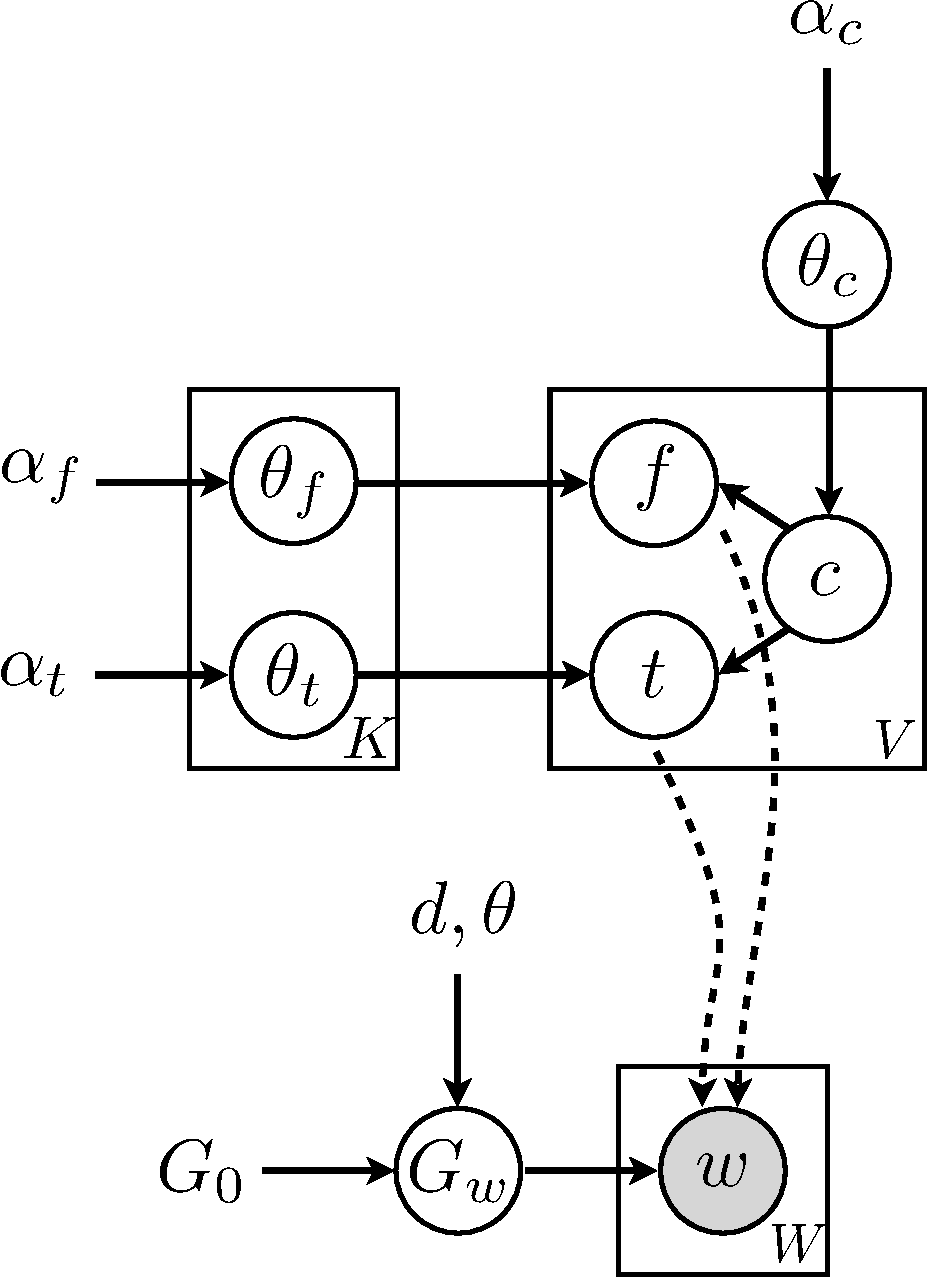
\includegraphics[width=0.5\textwidth]{fig/graph-model}
\caption{Baseline model}
\label{fig:graph-model}
\end{figure}

This baseline generative process is summarized in plate notation in
Figure~\ref{fig:graph-model}. Note that, although this breakdown of
morphology into stem and suffixes is reasonable for English, it is too
simplistic for languages with richer morphology. We therefore intend
to substitute the morpheme generation process with the following:
\begin{enumerate}
    \item Choose a class from a similar multinomial distribution with a Dirichlet prior
    \item Generate a stem conditioning on the class
    \item Choose a number of inflectional morphemes given a Poisson distribution specific to the class
    \item Generate a sequence of inflectional morphemes, either independently from a single multinomial or from a sequence model
\end{enumerate}

\subsection{Evaluation method}

We are not as interested in the final parameter values infered as much
as in the analyses produced for each word. We could measure the
perplexity of the model on held-out data, but we prefer to focus on
the core goal of the project and evaluate the stemming or segmentation
accuracy.

XXXXXXXXXXXXXXXXXXXXXXXXX TODO XXXXXXXXXXXXXXXXXXXXXXXXX
\begin{enumerate}
    \item splitting accuracy
    \item stemming accuracy (ability to map different variants to same word - precision/recall?)
\end{enumerate}

\subsection{Model Reparameterization}

The model described in \cite{goldwater2011} is a Pitman Yor process
mixture model; a generalization of a Dirichlet process mixture
model. With this in mind, we can then think of how the
reparameterization of DP mixture models presented in \cite{lovell2012} can be
used to reparameterize (and consequently paralellize) the model used
by \cite{goldwater2011} to perform unsupervised morphological
analysis.

There is a key difference between the purpose of the DP mixture model
as presented in \cite{lovell2012} and in \cite{goldwater2011} that
must be briefly discussed as it makes the reparameterization
non-trivial. \cite{lovell2012} discuss DP mixture models in the
context of an infinite mixture over Gaussian densities, where the
emphasis is not on the base distribution $H$, but rather on the
partition of the data that is induced by the CRP, and the means
(and/or variances) of the individual Gaussians that ``explain'' the
data assigned to the respective cluster.

The work in \cite{goldwater2011} can also be viewed as a DP mixture
model, but their work is cast in terms of a ``generator'' (the base
distribution $H$) and an ``adaptor'' (the process that allows
observations to be drawn without directly sampling from the the
generator). In the model of morphology that we have implemented the
adaptor is a Pitman Yor process. The important difference is the
emphasis on the base distribution $H$. That is, instead of $H$ being a
simple distribution over Gaussian mean parameters, for example, it is
actually a relatively sophisticated model of morphology. Therefore, we
are less interested in the partition of the data in this case (since
it essentially corresponds to word identities, and those are
observed), and are instead interested in the parameters of the
underlying base distribution $H$.

The reparameterization of the DP mixture model presented by
\cite{lovell2012} proposes a method for parallelizing the resampling
of seating arrangements, which is often the most expensive set of
operations in MCMC inference of DP mixture models (since we need to
reseat each sample in the dataset).

Our current implementation of the model presented in
\cite{goldwater2011} follows a relatively simple sampling scheme. We
initially iterate over all raw words in the corpus, sampling a table
from the CRP. If a word is assigned to an existing table, then we
simply increment the number of customers at the table and continue. If
the customer is chosen to start a new table, an analysis of the word
is sampled and the base model is incremented (i.e. given a class,
stem, and suffix, the multinomials in the base model $H$ are
incremented to account for the new observation). After the initial
iteration, we continue a fixed number of times through the sequence of
words. At each word, we first remove it from its table (performing any
table cleanup that is necessary), and then reseat it according to the
same procedure as explained for the first iteration.

Our current implementation mixes both the table assignment and
analysis sampling, which makes parallelization difficult if we wish to
use the reparameterization proposed by \cite{lovell2012}. The sampling
scheme proposed in \cite{goldwater2011}, however, separates the
simulation into two distinct steps. They first fix the assignment of
words to tables, and sample a new morphological analysis for the label
(word) of each table. In the second step, they fix the morphological
analyses assigned to tables, and resample the table assignments for
each word token in the dataset.

This alternative sampling strategy neatly divides the sampling
procedures for the morphological model $H$ and the CRP, which will
allow us to reparameterize the model according to the work in
\cite{lovell2012}, and perform parallel sampling for the second step
(table assignments).

Concretely, our sampling procedure will be changed to the
following. During the initial iteration, for each word token $w_n$ we
sample a supercluster from the Dirichlet multinomial defined by
$\boldsymbol{\mu}$, $\alpha$, and the previous supercluster
assignments:

\begin{align}
  s_{w_n} = i | \boldsymbol{\mu}, \alpha, \{s_{w_m}\}_{m=1}^{n-1} \sim
  \frac{\alpha \mu_i + \sum_{m=1}^{n-1} \mathbb{I}(s_{w_m} = i)}{\alpha + n - 1}
\end{align}

Conditioned on the supercluster chosen for the word, we then sample a
table from a CRP that is local to the supercluster. Since the local
CRPs allow the table assignments to be drawn independently of all
words in other superclusters, resampling tables in can be done in
parallel.

\cite{lovell2012} note that in the case of infinite Gaussian mixture
models, the parameters of each cluster can be done locally on each
compute node since the data that the cluster must account for is
completely present on that machine. In our case, however, we are not
interested in updating cluster specific parameters, but rather
parameters of the global morphological model $H$. Although we can
sample tables in parallel, we will likely need to collect sufficient
statistics from each cluster and coordinate global updates to $H$ when
resampling analyses. Designing an efficient and effective method for
managing these global model updates will be a primary challenge for us
during the second half of the project.

\section{Experiments}
\label{sec:experiments}


\subsection{Datasets}

We run the baseline model on the Wall Street Journal (WSJ) news data extracted from the Penn Treebank
and a discussion board (DB) data. The WSJ dataset is a standard corpus 
for which we have the gold standard morphological analysis while the DB dataset 
is chosen because of its typical net-speak characteristics. We see 
the usual spelling variations and some other board specific morphological
 changes in the DB dataset. The datasets are preprocessed to tokenize 
and for stop-word removal. A minimal stop-words 
list~\footnote{http://www.ranks.nl/resources/stopwords.html} containing 
the basic function words is used for stop-word removal.

To reproduce the experiments from \cite{goldwater2011}, only verbs from WSJ 
are given as input for the model. Since we don't have Part-of-Speech (POS)
 tags for the DB dataset, all the words after stop-word removal were 
given as input for the model. It can be assumed that the input in case of 
this dataset is both verbs and nouns as most function words are filtered 
through stop-word removal. This decision affects the quality of output 
from the model for the DB dataset which we'll discuss while doing a 
qualitative analysis of the model's output.

The input to the model is a sequence of word tokens. We generate this 
from both the datasets by going through each sentence and printing verbs 
in case of WSJ and non-stop-words in case of the DB dataset.

\subsection{Setup}

The Dirichlet hyper-parameters for classes, stems and suffixes 
$\alpha_{c}$, $\alpha_{t}$, $\alpha_{f}$ are set to 
$0.5$, $0.001$ and $0.001$ respectively. The discount parameter $d$ for the PYP is set 
to $0.1$ and the strength $\theta$ close to zero.
We vary the number of classes from 4 to 9 and run the sampler for 1000 
iterations. The entire model is run on both the datasets for 10 times 
for the above settings and the average time taken (seconds) is recorded.
This average time taken is the measure that we focus on and intend to 
improve in this work.

\subsection{Model performance}

Sample output from the baseline on the WSJ and DB datasets can be seen 
in Tables \ref{outputWSJ} and \ref{outputDB} respectively. The number 
of classes used for these outputs is 6 for WSJ and 8 for DB. The output
 has class, stem and suffix for each word. Words assigned the same class
 by the model are showed together in the tables. Average time taken by 
the model for various classes and datasets can be seen in 
Table~\ref{timeTable}. Average accuracy over 10 runs for WSJ is given 
in Table~\ref{accuTable}.


\begin{table*}[ht]
\begin{minipage}[b]{0.5\linewidth}\centering
\begin{tabular}{lccc}
\hline
Word & Class & Stem & Suffix \\
\hline
narrowed&3&narrow&ed \\
adjusted&3&adjust&ed \\
said&3&sai&d \\
estimated&3&estimate&d \\
has&3&ha&s \\
keeps&3&keep&s \\
providing & 4 & providing & \\
were&4&were& \\
hops&1&h&ops \\ 
revised&1&revis&ed \\
devastating&1&devastat&ing\\
outperforms&1&outperform&s\\
cover&5&cov&er \\
voting&5&votin&g \\
\hline
 \end{tabular}
\caption{\label{outputWSJ} Sample output from WSJ}
\end{minipage}
\begin{minipage}[b]{0.5\linewidth}\centering
\begin{tabular}{lccc}
\hline
  Word & Class & Stem & Suffix \\
\hline
many & 3 & man & y \\
died & 3 & di & ed \\
trade & 3 & trade &  \\
upping & 3 & upp & ing \\
laughin & 3 & laugh & in \\
numbers & 3 & number & s \\
amigos & 0 & amigo & s \\ 
ref & 0 & ref & \\
fonzworth & 4 & fonzworth & \\
ahahahaha & 4 & ahahahaha & \\
cowboys & 5 & cowboy & s \\
wastin & 5 & wastin & \\
accomplished & 7 & accomplished & \\
datshit & 7 & datshit & \\
\hline
 \end{tabular}
\caption{\label{outputDB} Sample output from DB}
\end{minipage}
\end{table*}

\begin{table}[ht]
\begin{minipage}[b]{0.5\linewidth}\centering
 \begin{tabular}{lcc}
  \hline
  \# Classes & WSJ & DB \\
  \hline
  4 & & \\
  5 & & \\
  6 & & \\
  7 & & \\
  8 & & \\
  9 & & \\
  \hline
 \end{tabular}
\caption{\label{timeTable}Average time (seconds) taken}
\end{minipage}
\begin{minipage}[b]{0.5\linewidth}\centering
 \begin{tabular}{lc}
  \hline
  \# Classes & Average accuracy \\
  \hline
  4 & \\
  5 & \\
  6 & \\
  7 & \\
  8 & \\
  9 & \\
  \hline
 \end{tabular}
\caption{\label{accuTable}Model accuracy on WSJ}
\end{minipage}
\end{table}

\subsection{Qualitative analysis}

\section{Conclusion}
\label{sec:conclusion}

\bibliographystyle{plain}
\bibliography{bibliography}

\end{document}
